\documentclass{article}
\usepackage{arxiv}

\usepackage[utf8]{inputenc}
\usepackage[english, russian]{babel}
\usepackage[T1]{fontenc}
\usepackage{url}
\usepackage{booktabs}
\usepackage{amsfonts}
\usepackage{nicefrac}
\usepackage{microtype}
\usepackage{lipsum}
\usepackage{graphicx}
\usepackage{natbib}
\usepackage{doi}



\title{Адаптивное сжатие в распределенной оптимизации}

\author{ Хафизов Фанис Адикович \\
	Физтех-школа Прикладной Математики и Информатики\\
	Московский Физико-Технический Институт\\
	г. Долгопрудный\\
	\texttt{khafizov.fa@phystech.edu} \\
	%% examples of more authors
	\And
	Безносиков Александр Николаевич \\
	Московский Физико-Технический Институт\\
	\texttt{https://anbeznosikov.github.io/} \\
	%% \AND
	%% Coauthor \\
	%% Affiliation \\
	%% Address \\
	%% \texttt{email} \\
	%% \And
	%% Coauthor \\
	%% Affiliation \\
	%% Address \\
	%% \texttt{email} \\
	%% \And
	%% Coauthor \\
	%% Affiliation \\
	%% Address \\
	%% \texttt{email} \\
}
\date{}

\renewcommand{\shorttitle}{Адаптивное сжатие}

%%% Add PDF metadata to help others organize their library
%%% Once the PDF is generated, you can check the metadata with
%%% $ pdfinfo template.pdf
\hypersetup{
pdftitle={Адаптивное сжатие в распределенной оптимизации},
% pdfauthor={David S.~Hippocampus, Elias D.~Striatum},
% pdfkeywords={First keyword, Second keyword, More},
}

\begin{document}
\maketitle

\begin{abstract}
В данной работе рассматривается проблема распределённого обучения больших моделей (например, современных нейросетей), когда вычисления необходимо распараллеливать между несколькими устройствами. Основная сложность в таких системах заключается в высокой стоимости коммуникации при передаче больших объёмов градиентов. Мы предлагаем семейство операторов \emph{адаптивного сжатия}, которые учитывают важность координат и тем самым снижают трафик, сохраняя качество сходимости. В экспериментальной части показано, что предлагаемые операторы могут работать не хуже классических вариантов \texttt{RandK} и \texttt{TopK}, а в ряде случаев достигают сопоставимого качества с \texttt{TopK}.
\end{abstract}

\keywords{Распределённая оптимизация \and Сжатие градиентов \and Нейронные сети \and Метод стохастического градиента}

\section{Введение}
Современные нейросетевые архитектуры требуют значительных вычислительных мощностей и объёмов памяти. Для ускорения обучения такие модели обычно тренируют на нескольких устройствах (GPU/TPU и т.\,д.), каждый из которых вычисляет градиенты на своей части данных. В итоге возникает проблема обмена градиентами между устройствами, так как полная пересылка всех координат может стать узким местом.

\textbf{Цель} данной работы~--- предложить новый подход к \emph{адаптивному} сжатию градиентов, основанный на идее взвешивания координат по их важности, и проверить его эффективность на задачах логистической регрессии и классификации изображений нейросетью.

\section{Связанные работы}
В литературе известно несколько типов операторов сжатия:
\begin{itemize}
\item \texttt{RandK}~--- случайный выбор $k$ координат из $d$;
\item \texttt{TopK}~--- выбор $k$ крупнейших по модулю координат.
\end{itemize}
Эти методы существенно сокращают объём передаваемых данных, однако могут приводить к смещённым оценкам градиента и замедлять сходимость. Поэтому активно исследуются \emph{смещённые} операторы сжатия, которые, с одной стороны, уменьшают трафик, а с другой~--- обладают хорошими свойствами сходимости при грамотном учёте структуры данных.

\section{Постановка задачи}
Рассмотрим задачу минимизации функции
\begin{equation}
  \label{eq:distributed_optimization}
  \min_{x \in \mathbb{R}^d}\left\{f(x) := \frac{1}{n}\sum\limits_{i = 1}^n f_i(x) \right\},
\end{equation}
где $n$~--- число устройств (воркеров), $f_i(x)$~--- функция потерь на $i$-м устройстве. Типичная схема \emph{распределённого} градиентного спуска (DCGD) с учётом сжатия выглядит так:
\begin{equation}
  x^{k+1} = x^k - \frac{\eta}{n} \sum_{i=1}^n \mathcal{Q}\bigl(\mathcal{C}_i^k(\nabla f_i(x^k))\bigr),
\end{equation}
где $\mathcal{C}_i^k$~--- оператор сжатия на $i$-м устройстве в момент времени $k$, а $\mathcal{Q}$~--- опциональный оператор квантизации (например, округление до ближайшей степени двойки).
\section{Предлагаемый метод}
\subsection{Идея важности координат}
Ключевая идея~--- ввести \emph{вектор важности} $w \in [0, 1]^d$, который присваивает каждой координате некоторый «вес»:
\[
  w^k = \arg\min_{w \in \Delta_d} f\bigl(x^k - \eta\, (w \odot \nabla f(x^k))\bigr),
\]
где $\Delta_d = \{\, w \in \mathbb{R}^d \,\vert\, w_i \ge 0, \sum_i w_i = 1 \}$ и $\odot$ обозначает поэлементное умножение. Оптимизацию по $w$ можно проводить методом зеркального спуска. После нахождения $w^k$ оператор сжатия учитывает не просто значение координаты, а её «важность».

\subsection{Примеры операторов}
Мы предлагаем несколько вариантов на базе $w$:
\begin{itemize}
\item \textbf{MD Stochastic:} случайный отбор $k$ координат с вероятностью $w_i$;
\item \textbf{MD Greedy:} отбор $k$ координат с наибольшими $w_i$;
\item \textbf{MD Greedy Weighted:} масштабирование координат $x_i$ дополнительно на $w_i$;
\item \textbf{MD Weighted Greedy:} выбор по наибольшим значениям $|w_i \, x_i|$.
\end{itemize}
В результате получается \emph{смещённая} оценка градиента, однако весовые коэффициенты $w$ помогают выделять более важные координаты.

\section{Эксперименты}
Мы провели эксперименты на задаче логистической регрессии (\texttt{mushrooms} датасет) и на задаче классификации изображений (\texttt{CIFAR10} с моделью ResNet18).

\subsection{Логистическая регрессия}
На Рис.~\ref{fig:logreg} приведены результаты для доли передаваемых координат $k/d = 0.2$. Виден выигрыш операторов, учитывающих важность, по сравнению с \texttt{RandK}.
\begin{figure}[h]
\centering
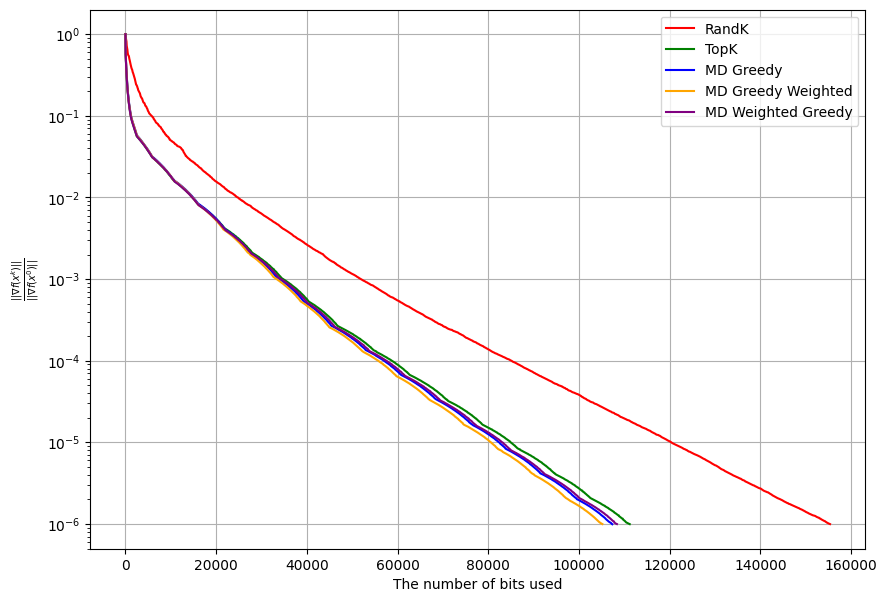
\includegraphics[width=0.6\textwidth]{../figures/LogReg}
\caption{Сходимость алгоритма логистической регрессии (датасет mushrooms).}
\label{fig:logreg}
\end{figure}

\subsection{Классификация (ResNet18 на CIFAR10)}
На Рис.~\ref{fig:cifar10} показаны результаты обучения ResNet18. Предлагаемые методы демонстрируют качество, близкое к \texttt{TopK}, но требуют меньше объёма передачи данных по сравнению с полной пересылкой.
\begin{figure}[h]
\centering
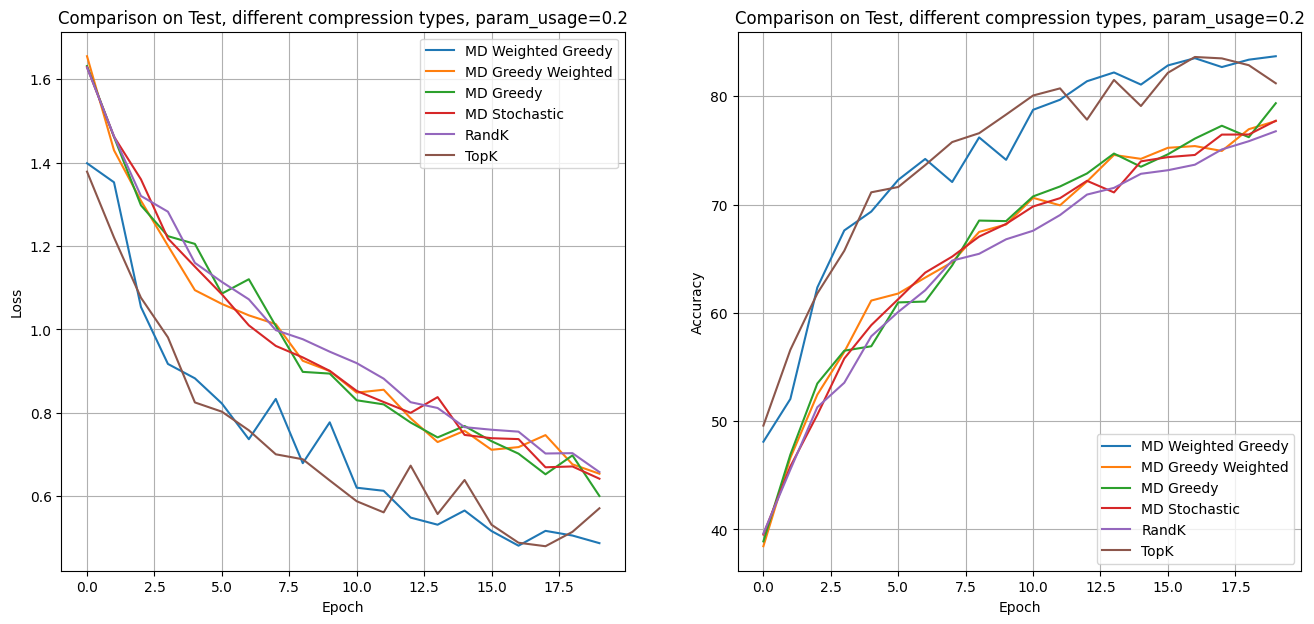
\includegraphics[width=0.6\textwidth]{../figures/ResNet_CIFAR10}
\caption{Сходимость при обучении ResNet18 на CIFAR10 с долей $k/d = 0.2$.}
\label{fig:cifar10}
\end{figure}

\section{Выводы}
\begin{itemize}
\item Введено семейство операторов сжатия, использующих \emph{вектор важности} $w$.
\item Эксперименты показывают, что данные операторы, особенно \texttt{MD Weighted Greedy}, дают сравнимую сходимость с классическим \texttt{TopK}.
\item В дальнейших исследованиях планируется:
  \begin{enumerate}
  \item Улучшать качество сходимости за счёт дополнительной теоретической настройки параметров;
  \item Расширять эксперименты на более сложных нейросетевых архитектурах.
  \end{enumerate}
\end{itemize}

\end{document}
